\section{Problematiche} \label{sec:prob}
In questa sezione verranno descritti brevemente per chiarezza i problemi che il sistema si propone di risolvere, i quali quindi sono stati oggetto di studio per lo stagista che ha dovuto analizzarli e ricercarne una soluzione.
\subsection{Camera Calibration} \label{sec:camcalib}
Per \textit{camera calibration} si intende la procedura volta a calcolare la relazione matematica tra le coordinate di un punto posizionato nello spazio e la sua proiezione sull'\textit{image plane} di una telecamera. \\

\subsubsection{Intrinsics parameters}
La visione origina dall'individuazione della luce nell'ambiente. La luce parte da una qualche sorgente per poi viaggiare nello spazio fino ad incontrare un oggetto, in quel momento buona parte della luce viene assorbita, la parte che non viene assorbita viene riflessa e determina il colore dell'oggetto. \\

Il modello più semplice disponibile per la rappresentazione di una telecamera è il cosiddetto \textit{pinhole camera model}. In tale modello la luce arriva da un oggetto distante, ma solo un singolo raggio entra per ogni particolare punto. Tale punto viene proiettato su di una superficie. Ciò comporta che l'immagine presente sull'\textit{image plane} è sempre a fuoco, e la sua dimensione dipende dalla distanza della sorgente della luce (\textit{focal lenght}).

Si può vedere in figura ~\ref{fig:calib1}) una rappresentazione di tale modello.
\begin{figure}[htpb] 
\centering 
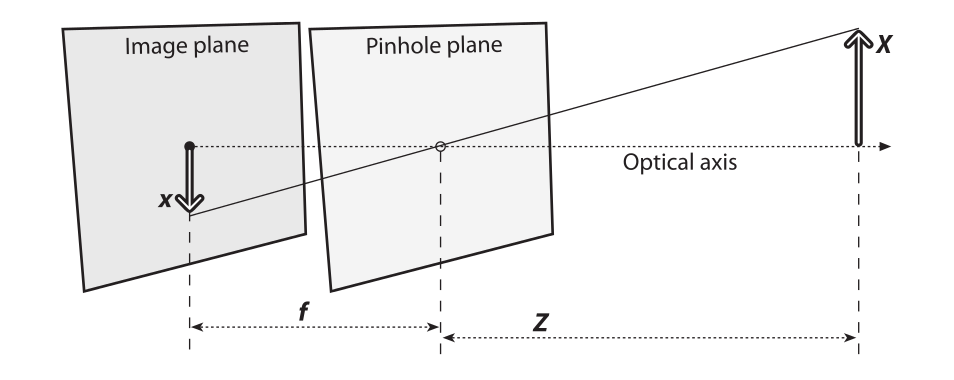
\includegraphics[scale=0.4]{./images/calib1.png} 
\caption{Rappresenzazione di un pinhole camera model} 
\label{fig:calib1}
\end{figure} 

In tale figura \em{f} è la \em{focal lenght} della telecamera, \textit{Z} la distanza tra oggetto e telecamera, \em{X} la dimensione dell'oggetto e \em{x} l'immagine dell'oggetto proiettata sul piano. \\ Il modello appena descritto può essere reinterpretato come in figura ~\ref{fig:calib2} 
\begin{figure}[htpb] 
\centering 
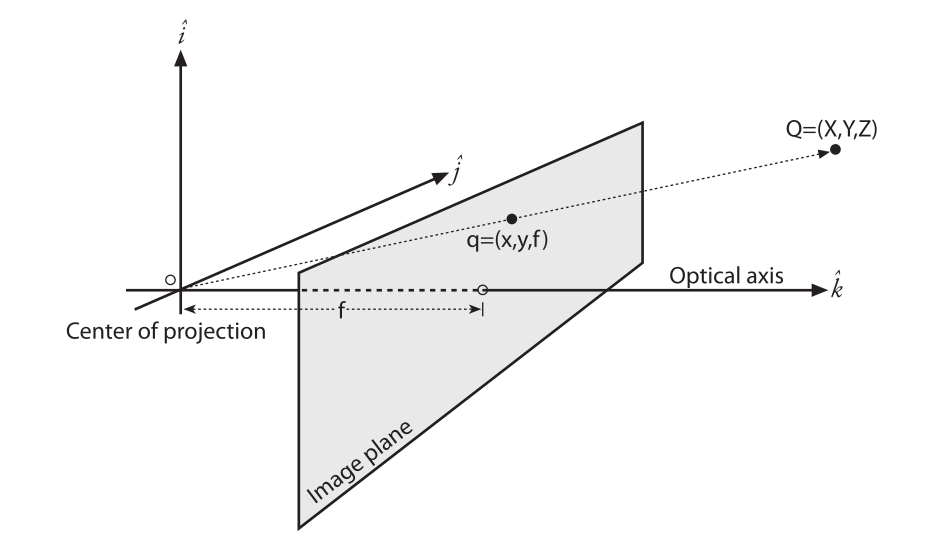
\includegraphics[scale=0.4]{./images/calib2.png} 
\caption{Rappresenzazione di un pinhole camera model rovesciato} 
\label{fig:calib2}
\end{figure} 

nella quale sono stati rovesciati il punto di \textit{pinhole} e l'\textit{image plane}. Ciò ci permette di semplificare le relazioni che valgono tra i punti dell'oggetto e le loro proiezioni. Infatti ora è più chiara la similarità dei triangoli, inoltre l'immagine non è più capovolta come era in figura ~\ref{fig:calib1}. In tale visione vanno aggiunti altri due nuovi parametri \em{c\textsubscript{x} }e \em{c\textsubscript{y}} per considerare un eventuale \textit{displacement} del centro delle coordinate sull'\textit{image plane}, dovuto alla possibilità che il centro del chip (della telecamera) non risieda esattamente sopra l'asse indicato in figura ~\ref{fig:calib2} come \textit{optical axis}. \\ \\
In tale visualizzazione c'è una semplice relazione che mappa i punti \em{Q\textsubscript{i}} nello spazio (coordinate (\em{X\textsubscript{i}},\em{Y\textsubscript{i}},\em{Z\textsubscript{i}})) nei punti sul piano di proiezione (coordinate (\em{x\textsubscript{i}},\em{y\textsubscript{i}})), tale relazione è chiamata \textit{projective transform}. Viene riportata in figura ~\ref{fig:calib3}
\begin{figure}[htpb] 
\centering 
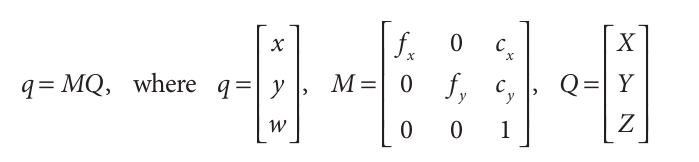
\includegraphics[scale=0.4]{./images/calib3.png} 
\caption{Espressione matematica di una relazione projective transform} 
\label{fig:calib3}
\end{figure} 

Tale modello è utile per capire la meccanica della geometria tridimensionale di visione, ma non è utilizzato nella realtà perche presenta dei limiti. Esso infatti in pratica porterebbe a una frequenza di generazione dei frame molto lenta, dovuta alla bassa quantità di luce che riesce a passare attraverso un \textit{pinhole}. Per ottenere una maggiore quantità di luce e quindi un maggior rapporto di frame/secondo è necessario utilizzare una lente, che consente di raccogliere molta più luce e di curvarla in maniera che converga nel punto di projection. Lo svantaggio di utilizzare una lente è che viene introdotta la \textit{distortion}. \\ \\

\subsubsection{Distortion parameters}

La \textit{lens distortion} si può dividere in due principali tipi:
\begin{enumerate}
	\item \textit{radial distortion}
	\item \textit{tangential distortion}
\end{enumerate}

La prima è un risultato della forma fisica della lente. Le lenti infatti tendono a distorcere i pixel vicini ai bordi dei frame, tale fenomeno è chiamato "barrel effect". Viene riportata in figura ~\ref{fig:calib4} uno schema che aiuta l'intuizione del motivo per cui tale fenomeno si verifica.
\begin{figure}[htpb] 
\centering 
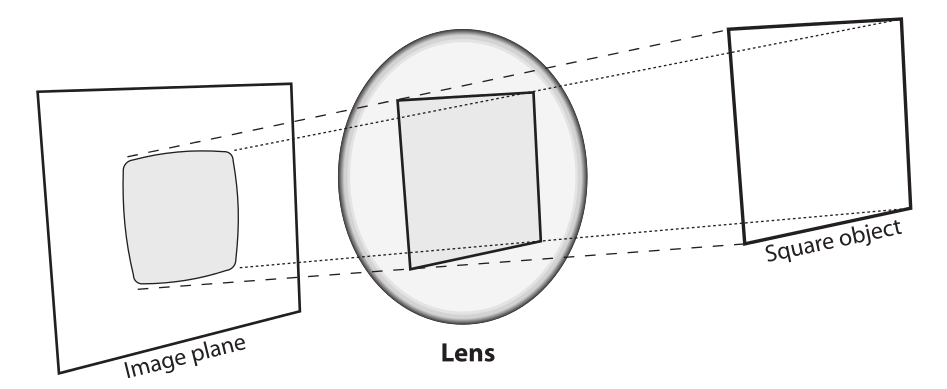
\includegraphics[scale=0.3]{./images/calib4.png} 
\caption{Radial distortion effect} 
\label{fig:calib4}
\end{figure} 
\\ \\
La seconda è un risultato dei difetti di assemblaggio che portano la lente a non essere perfettamente parallela all'\textit{image plane}. Si riporta un immagine che evidenzia tale fenomeno in figura ~\ref{fig:calib5}.
\begin{figure}[htpb] 
\centering 
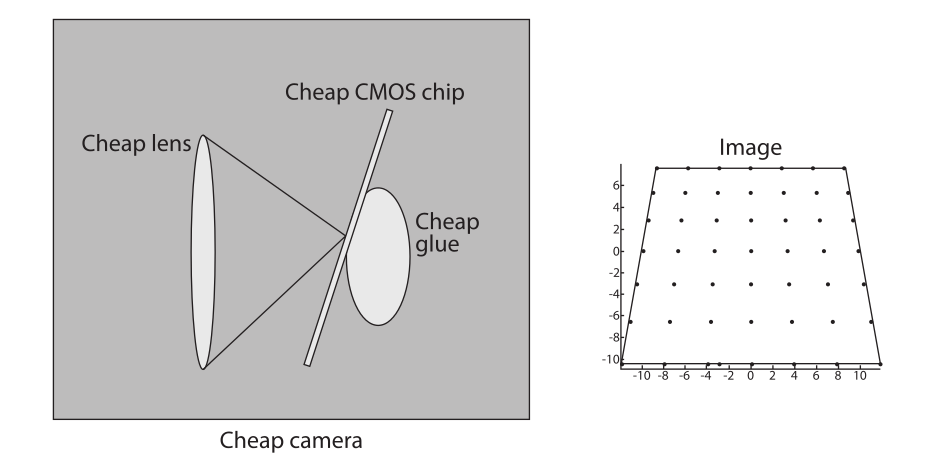
\includegraphics[scale=0.3]{./images/calib5.png} 
\caption{Tangential distortion effect} 
\label{fig:calib5}
\end{figure} 

\subsubsection{Calibrazione}

Ora che è stato descritto come identificare a livello matematico le proprietà \textit{intrinsics} e \textit{distortion} possiamo vedere le tecniche con le quali si prendono in considerazione tali parametri per correggere i frame catturati dalla telecamera.\\
Le tecniche di calibrazione si basano sul seguente criterio: viene esposto mostrato alla camera un oggetto di cui si conosce la struttura, e si valutano le differenze tra le caratteristiche dell'oggetto catturato dalla camera (quindi proiettato sull'\textit{image plane}) con le sue note caratteristiche fisiche. \\Per ogni immagine che una telecamera cattura di un oggetto, è possibile descrivere la sua posizione rispetto al sistema di coordinate della telecamera in termini di rotazione e traslazione. Possiamo quindi definire una relazione tra la posizione nello spazio di un oggetto e le sue coordinate nel frame catturato dalla telecamera. Combinando tale relazione con le correzioni derivanti dai parametri di \textit{intrinsics} si ottiene un sistema di equazioni che risolto rappresenta la soluzione al problema della calibrazione.\\
In linea di principio qualsiasi oggetto può essere usato ai fini di tale operazione, ma è pratico utilizzare un oggetto che presenta caratteristiche regolari (pattern). All'interno del progetto verrà utilizzata una immagine di una scacchiera con dimensioni (numero di celle) predefinite.  \\
Si potrà vedere come OpenCV offre un API di alto livello per la soluzione del problema della calibrazione con l'utilizzo di una scacchiera.

\subsection{Tracking data transformation}

\subsubsection{Homography matrix}

\subsubsection{Qt coordinate system}


\subsection{Qt gradients}
